\section{Introduction} \label{intro}

Starting of DC motors can be tricky in many applications. Basic modelling of DC motors can be given in following figure and equations:

\begin{figure}[ht!]
    \centering
    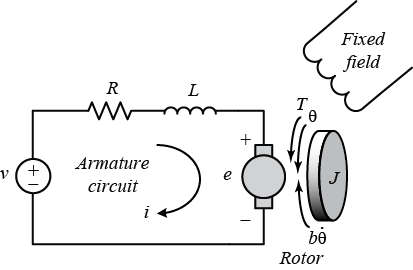
\includegraphics{Figures/DC_motor_model.png}
    \caption{Simplified DC-machine model.}
    \label{fig:DC-mmotor}
\end{figure}

\begin{equation}
    E_{emf} = K_e\times\omega
\end{equation}

\begin{equation}
    T_e = K_t\times I
\end{equation}

where $K_e$ and $K_t$ are machine constants. $\omega$ being the machine rotational speed, at the starting operation, it is obviously zero. Therefore if we apply a high DC voltage at the starting instant, the DC machine will draw high amounts of currents which can damage the device, permanently. To prevent this possibility, one can start the DC motor in a proper way, not applying a step voltage (rated) to the motor terminals, but rather applying a voltage that increases properly up to the rated value. This kind of operation is called \textit{soft start} and it is helpful  in prolonging the lifetime of the DC motor. In this project, our aim is to make a rectifier controller that is capable of soft-starting the DC motor. Requirements of the controllers and details of the motor of interest are given on course Github web page.\cite{course_git} These will also be used in the following sections of the report.

There are different types of topologies for this purpose of soft start. Some of the common topologies are discussed and evaluated on the issues of efficiency, operation regions and ratings, component availability, thermal and mechanical considerations, etc. on the design decision in \ref{design}. Also, the reasons behind the  design selection of Hard-time Regulators are given in the same section. Selected topology is simulated on computer software programs and the performance of the topology is investigated in the related section \ref{simulations}. Also, possible components that are commercially available and appropriate for the design, are issued on the component selection (see \ref{component}). Summary and future considerations on the design are given in the conclusion.(see \ref{conclude})